\chapter{API del cockpit}
\label{apendiceC}
\lhead{Apéndice C.}

Es \textbf{importante} considerar que la API del software aquí plasmado se corresponde al que se encuentra ejecutándose en el OpenROV, ya que difiere de los repositorios que pueden ser descargados del github oficial.

\section{Servidor de Node.js}

\subsection{API}
Los módulos creados para node.js que definen la API del cockpit se encuentran en:

\begin{verbatim}
$ cd /opt/openrov/cockpit/src/lib    
\end{verbatim} 
Como interactúan o se relacionan entre sí se muestra en los siguientes diagramas. 

\begin{figure}[H]
    \centering
    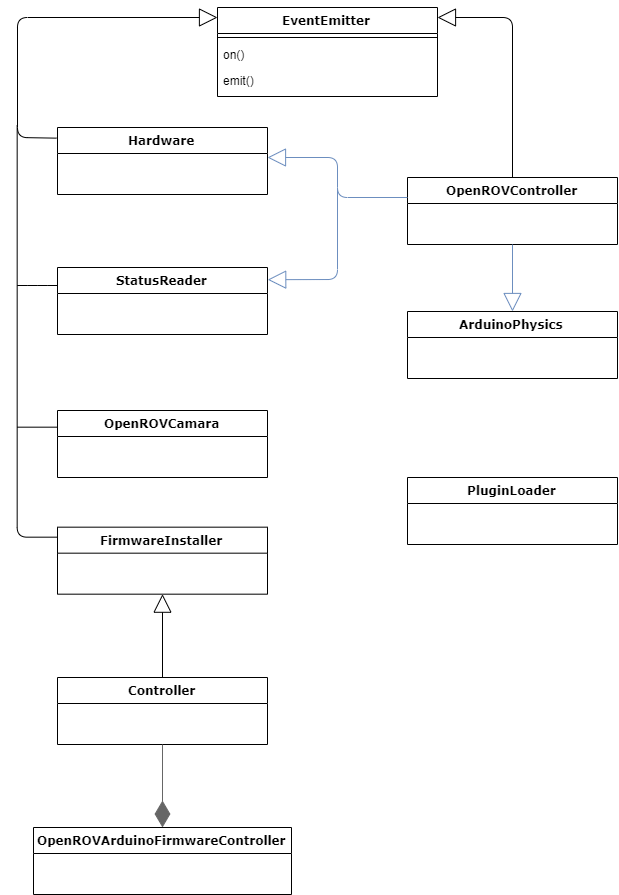
\includegraphics[scale=0.65]{partes/ImgSophia/ApendiceC/ApiCockpit1.png}
    \caption{API en general de los módulos del Cockpit}
    \label{fig:APICockpit1}
\end{figure}

\begin{figure}[H]
    \centering
    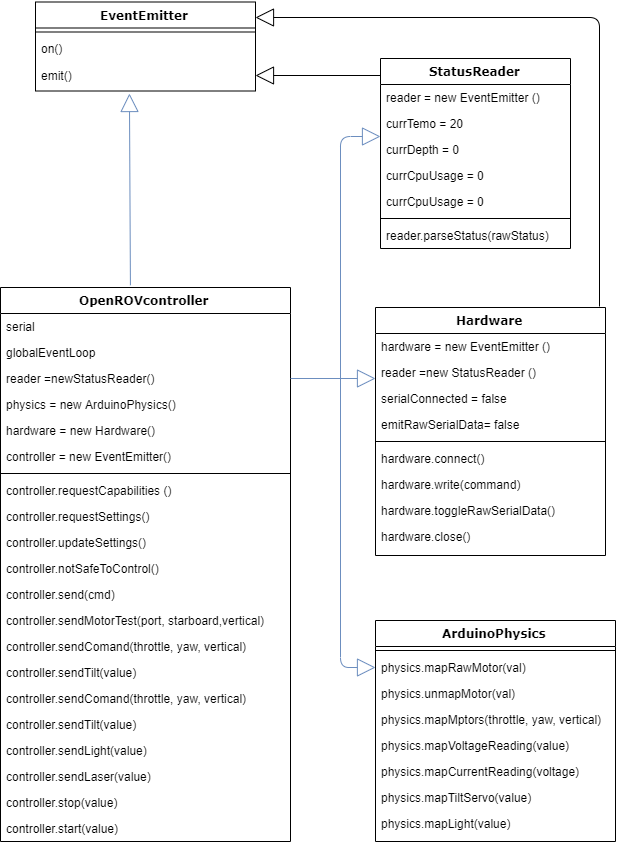
\includegraphics[scale=0.65]{partes/ImgSophia/ApendiceC/ApiCockpit2.png}
    \caption{Estructura de algunas módulos 1}
    \label{fig:Apicockpit2}
\end{figure}

\begin{figure}[H]
    \centering
    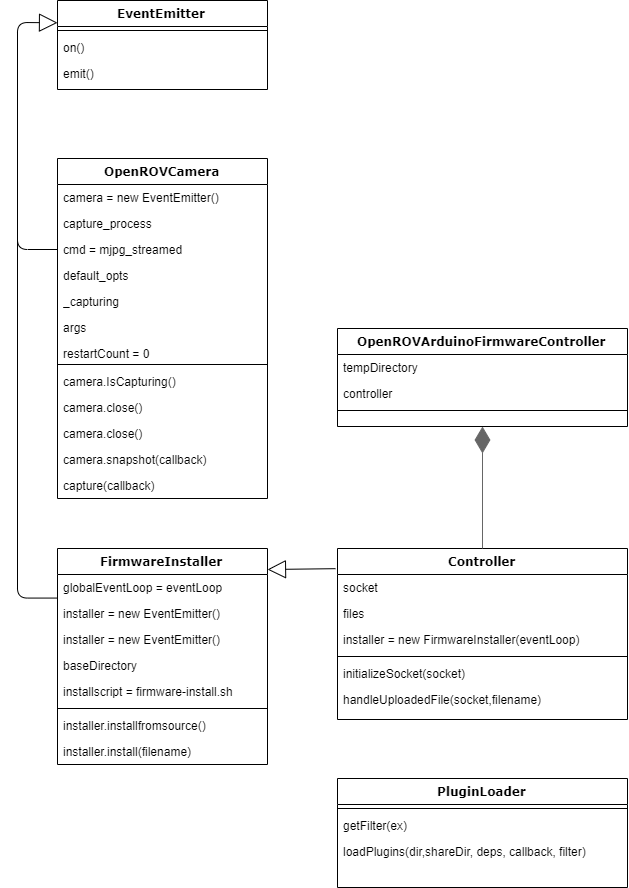
\includegraphics[scale=0.63]{partes/ImgSophia/ApendiceC/ApiCockpit3.png}
    \caption{Estructura de algunos módulos 2}
    \label{fig:Apicockpit3}
\end{figure}

%% FLOWCHARTS

\begin{figure}[H]
    \centering
    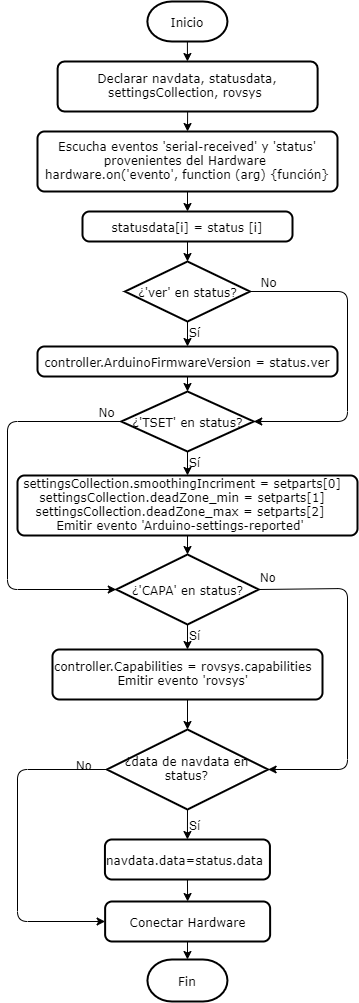
\includegraphics[scale=0.63]{partes/ImgSophia/ApendiceC/DiagramaOpenROVController.png}
    \caption{Diagrama del proceso en OpenROVController.js}
    \label{fig:DiagOROVController}
\end{figure}

\begin{figure}[H]
    \centering
    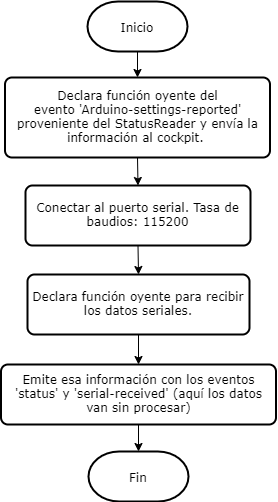
\includegraphics[scale=0.63]{partes/ImgSophia/ApendiceC/DiagramaHardware.png}
    \caption{Diagrama del proceso en Hardware.js}
    \label{fig:DiagHardware}
\end{figure}

\begin{figure}[H]
    \centering
    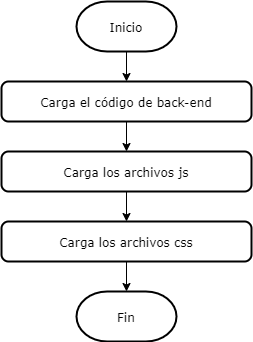
\includegraphics[scale=0.63]{partes/ImgSophia/ApendiceC/DiagramaPluginLoad.png}
    \caption{Diagrama del proceso en PluginLoader.js}
    \label{fig:DiagPluginLoader}
\end{figure}




\subsubsection{cockpit.js}

\par La integración final de esos módulos ocurre en el archivo donde se ejecuta el servidor de node.js:

\begin{verbatim}
$ /opt/openrov/cockpit/src/cockpit.js    
\end{verbatim} 

\par Aquí se definen también el intervalo de tiempo para agarrar los $frames$, que se ajusta con la variable DELAY (está en milisegundos) y la variable $deps$.

\begin{figure}[H]
    \centering
    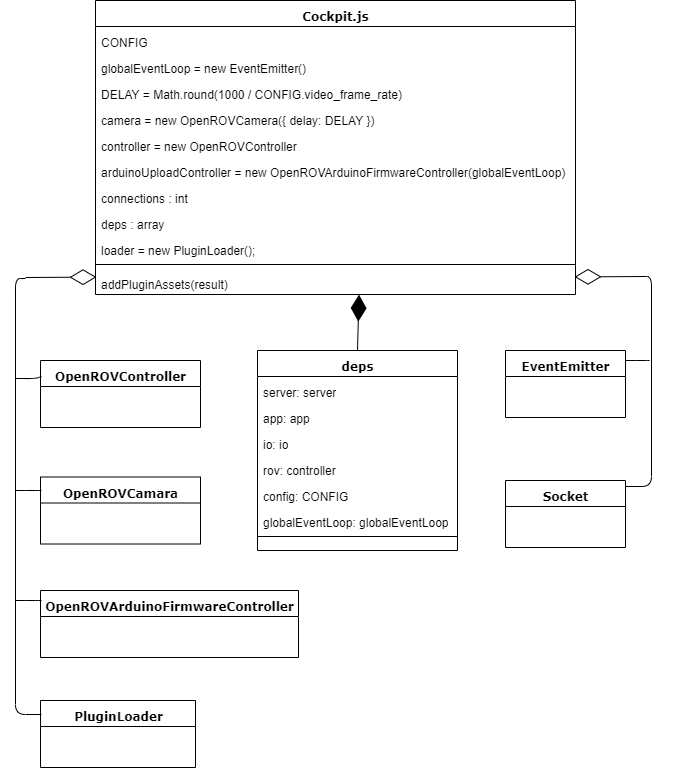
\includegraphics[scale=0.60]{partes/ImgSophia/ApendiceC/ApiCockpitjs4.png}
    \caption{API del cockpit, servidor de Node.js}
    \label{fig:Apicockpit4}
\end{figure}

\begin{figure}[H]
    \centering
    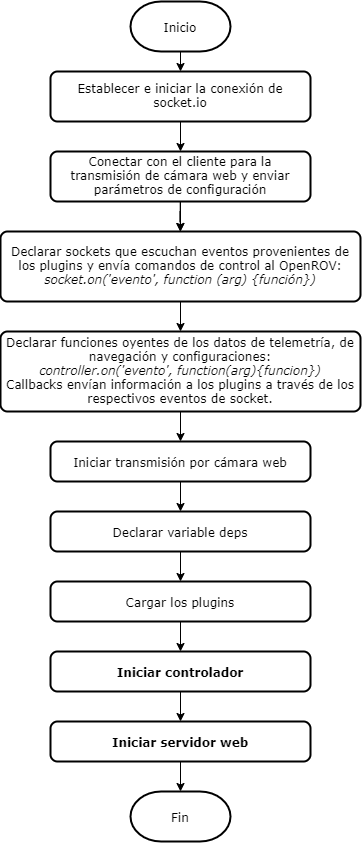
\includegraphics[scale=0.73]{partes/ImgSophia/ApendiceC/DiagramaCockpit.png}
    \caption{Diagrama del proceso del servidor de Node.js}
    \label{fig:DiagCockpit}
\end{figure}

\subsection{Plugins}

\subsubsection{ROVpilot}

\begin{itemize}
    \item \textit{rovpilot.js}: en este archivo, a través de un evento 
    emitido, se realiza el registro o las asignaciones de los valores de entrada que permiten el control del OpenROV, respondiendo a la sintaxis establecida en:
\end{itemize}


\begin{verbatim}
    cd /opt/openrov/cockpit/src/system-plugins/input-controller
\end{verbatim}
\par Y que se muetsra a continuación
\begin{verbatim}
    self.cockpit.extensionPoints.inputController.register(
        {
        name: "example.keyBoardMapping",
        description: "Example for keymapping.",
        defaults: { keyboard: 'alt+0', gamepad: 'X' },
        down: function() { console.log('0 down'); },
        up: function() { console.log('0 up'); }
        });
\end{verbatim}

Las siguientes tablas muestran la descripción de esos eventos emitidos desde el plugin del navegador y declarados de la forma:
\begin{verbatim}
    rov.cockpit.emit ('evento', valor)
\end{verbatim}

\begin{table}[H]
\caption {Comandos de entrada por teclado para controlar el ROV desde el cockpit. Los \textbackslash{} en la columna \textbf{valor} implican que la función no recibe ningún argumento } 
\label{tab:KeyboardRovpilot}
\centering
\footnotesize
\begin{tabular}{@{}lclc@{}}
\toprule
\textit{\textbf{name}}            & \multicolumn{1}{l}{\textit{\textbf{keyboard}}} & \textbf{evento}              & \multicolumn{1}{l}{\textbf{valor}} \\ \midrule
rovPilot.laserToggle              & l                                              & rovpilot.toggleLasers        & \textbackslash{}                   \\
rovPilot.adjustLights\_increment  & p                                              & rovpilot.adjustLights        & 0.1                                \\
rovPilot.adjustLights\_decrement  & o                                              & rovpilot.adjustLights        & -0.1                               \\
rovPilot.toggleLights             & i                                              & rovpilot.toggleLights        & \textbackslash{}                   \\
rovPilot.adjustCameraTilt\_down   & z                                              & rovpilot.adjustCameraTilt    & -0.1                               \\
rovPilot.adjustCameraTilt\_centre & a                                              & rovpilot.setCameraTilt       & 0                                  \\
rovPilot.adjustCameraTilt\_up     & q                                              & rovpilot.adjustCameraTilt    & 0.1                                \\
rovPilot.incrementPowerLevel      &                                                & rovpilot.incrimentPowerLevel & \textbackslash{}                   \\
rovPilot.moveForward              & arriba                                         & rovpilot.setThrottle         & 1                                  \\
rovPilot.moveBackwards            & abajo                                          & rovpilot.setThrottle         & -1                                 \\
rovPilot.moveLeft                 & izquierda                                      & rovpilot.setYaw              & -1                                 \\
rovPilot.moveRight                & derecha                                        & rovpilot.setYaw              & 1                                  \\
rovPilot.moveUp                   & shift                                          & rovpilot.setLift             & -1                                 \\
rovPilot.moveDown                 & ctrl                                           & rovpilot.setLift             & 1                                  \\
rovPilot.powerLevel1              & 1                                              & rovpilot.powerLevel          & 1                                  \\
rovPilot.powerLevel2              & 2                                              & rovpilot.powerLevel          & 2                                  \\
rovPilot.powerLevel3              & 3                                              & rovpilot.powerLevel          & 3                                  \\
rovPilot.powerLevel4              & 4                                              & rovpilot.powerLevel          & 4                                  \\
rovPilot.powerLevel5              & 5                                              & rovpilot.powerLevel          & 5                                  \\
rovPilot.powerOnESC               & {[}                                            & rovpilot.powerOnESCs         & \textbackslash{}                   \\
rovPilot.powerOffESC              & {]}                                            & rovpilot.powerOffESCs        & \textbackslash{}                   \\
rovPilot.toggleHeadingHold        & m                                              & rovpilot.toggleholdHeading   & \textbackslash{}                   \\
rovPilot.toggleDepthHold          & n                                              & rovpilot.toggleholdDepth     & \textbackslash{}                  \\ \bottomrule
\end{tabular}
\end{table}

\begin{table}[H]
\caption {Entradas a través del gamepad para controlar el ROV. Los \textbackslash{} en la columna \textbf{valor} implican que la función no recibe ningún argumento } 
\label{tab:GamepadRovpilot}
\centering
\footnotesize
\begin{tabular}{@{}lclc@{}}
\toprule
\multicolumn{1}{c}{\textit{\textbf{name}}} & \textit{\textbf{gamepad}} & \multicolumn{1}{c}{\textbf{evento}} & \textbf{valor}   \\ \midrule
rovPilot.adjustLights\_increment           & DPAD\_UP                  & rovpilot.adjustLights               & 0.1              \\
rovPilot.adjustLights\_decrement           & DPAD\_DOWN                & rovpilot.adjustLights               & -0.1             \\
rovPilot.adjustCameraTilt\_down            & A                         & rovpilot.adjustCameraTilt           & -0.1             \\
rovPilot.adjustCameraTilt\_centre          & B                         & rovpilot.setCameraTilt              & 0                \\
rovPilot.adjustCameraTilt\_up              & Y                         & rovpilot.adjustCameraTilt           & 0.1              \\
rovPilot.moveThrottle                      & LEFT\_STICK\_Y            & rovpilot.setThrottle                & 1*v              \\
rovPilot.moveYaw                           & LEFT\_STICK\_X            & rovpilot.setYaw                     & v                \\
rovPilot.moveLift                          & RIGHT\_STICK\_Y           & rovpilot.setLift                    & 1*v              \\
rovPilot.toggleDepthHold                   & X                         & rovpilot.toggleholdDepth            & \textbackslash{} \\ \bottomrule
\end{tabular}
\end{table}

\subsubsection{Otros Plugins}

Además de ROVpilot, que representa el plugin dedicado al control del OpenROV, otros plugins también poseen mapeos de comandos de entrada por teclado o gamepad que gestionan ciertas características de la interfaz del cockpit, y se presentan a continuación:

\begin{table}[H]
\caption {Entradas a través del gamepad para controlar el ROV. Los \textbackslash{} en la columna \textbf{valor} implican que la función no recibe ningún argumento } 
\label{tab:OtrosPlugins}
\centering
\footnotesize
\begin{tabular}{@{}llcl@{}}
\toprule
\multicolumn{1}{c}{\textbf{Plugin}} & \multicolumn{1}{c}{\textit{\textbf{name}}} & \textit{\textbf{key/gamepad}} & \multicolumn{1}{c}{\textbf{Descripción}}                                      \\ \midrule
\multirow{2}{*}{altservo.js}        & altservo.servoup                           & alt+q                         & Incrementar servo                                                             \\ \cmidrule(l){2-4} 
                                    & altservo.servodown                         & alt+z                         & Decrementar servo                                                             \\ \midrule
blackbox.js                         & blackbox.record                            & r                             & \begin{tabular}[c]{@{}l@{}}Grabar los datos \\ de telemetría\end{tabular}     \\ \midrule
flybywire.js                        & flyByWire.toggle                           & g                             & Fly by Wire                                                                   \\ \midrule
fpscounter.js                       & fpsCounter.toggleFpsCounter                & f                             & \begin{tabular}[c]{@{}l@{}}Conmutar FPS\\  de video\end{tabular}              \\ \midrule
\multirow{3}{*}{headsup-menu.js}    & headsupMenu.show                           & e                             & Menú "Heads up"                                                               \\ 
                                    & headsupMenu.next                           & c                             & Elemento sig.                                                                 \\ 
                                    & headsupMenu.prev                           & d                             & Elemento prev.                                                                \\ \midrule
\multirow{3}{*}{lights.js}          & lights.keyBoardMapping                     & alt+i                         &                                                                               \\ 
                                    & lights.keyBoardMapping                     & alt+p                         &                                                                               \\ 
                                    & lights.keyBoardMapping                     & alt+o                         &                                                                               \\ \midrule
photocapture.js                     & photoCapture.takeSnapshot                  & c                             & \begin{tabular}[c]{@{}l@{}}Captura imagen \\ actual del video\end{tabular}    \\ \midrule
serial-monitor.js                   & serialMonitor.toggleSerialMonitor          & u                             & \begin{tabular}[c]{@{}l@{}}Muestra/oculta \\ el monitor serial\end{tabular}   \\ \midrule
\multirow{5}{*}{tankcontrol.js}      & tankcontrol.toggleTankControl              & t                             & \begin{tabular}[c]{@{}l@{}}Activa/desactiva \\ control de tanque\end{tabular} \\  
                                    & rov.controlNames.leftLift                  & LEFT\_STICK\_X                &                                                                               \\  
                                    & rov.controlNames.portThrottle              & LEFT\_STICK\_Y                &                                                                               \\  
                                    & rov.controlNames.rightLift                 & RIGHT\_STICK\_X               &                                                                               \\ 
                                    & rov.controlNames.starboardThrottle         & RIGHT\_STICK\_Y               &                                                                               \\ \midrule
telemetry.js                        & telemetry.cycleTextColor                   & h                             & \begin{tabular}[c]{@{}l@{}}Cambiar color \\ texto telemetría\end{tabular}     \\ \bottomrule
\end{tabular}
\end{table}